\section{Rolling Road}
The Rolling Road's function is to test a subjects efficiency, at a specified torque or force. To do so it has to measure both the mechanic and electric power usage and calculate the efficiency based on those numbers.\\


To communicate with the Rolling Road a serial connection can be established with a USB-stick. Where the Rolling Road will feedback information from all sensors, and calculation of power and efficiency.\\ The serial connection can also be used to change different parameters like the wanted torque or PID parameter. It is also possible to make a calibration.

\subsection{Design}
The rolling road is made in c. because it is the only option where is beside Assembly, the architecture are design as a objective program with classes. But because c don't have classes and not a objective programming language. Header files with function prototypes was made instead. 

Because it is easier to design it as a objective program. To design the solution a class diagram was made see Rolling road documentation \cite{RR}.\\

The design of Rolling Road consist of three things: regulating, measure and communication. Where all these work together.\\

\subsection{Implementation}
In the implementation another problem was made clear, the measurements of sensors and the calculation were very time critical. To get a better overview over the flow, a flow-diagram was made see \vref{fig:data_flow_diagram}.

The flow-diagram gives a better overview of the Rolling Road and how data from the sensor comes to both the Regulator and are send over the serial connection.

The different signals from the sensors goes though a couple of steps before they are calculated and passed on. To save as much CPU time as possible DMA is implemented in the torque-sensor because it is the most time critics sensor. Also because it is the feedback of the regulator.  

 Where are implemented some decimation filter in the design, because the sensor are measured with a high sample frequency around 50 kSample/s. Where the PID regulator only runs with 2 kSample/s and the data transmitting rate is around 2-100 Sample/s (the rate can be change with a re-compiling).
 
There is also implemented a small exponential moving average filter, that smooths all data before sending to the control unit.  

To implement the calibration first it set the exponential filter alpha value to the LSB (ca. $ \alpha = 0.004 $), after what it will wait for a few seconds and read from the sensor and use the value as a offset value. After it has finish it will reset the alpha value back again and saved the offset values. 

\begin{figure}[H]
	\centering
	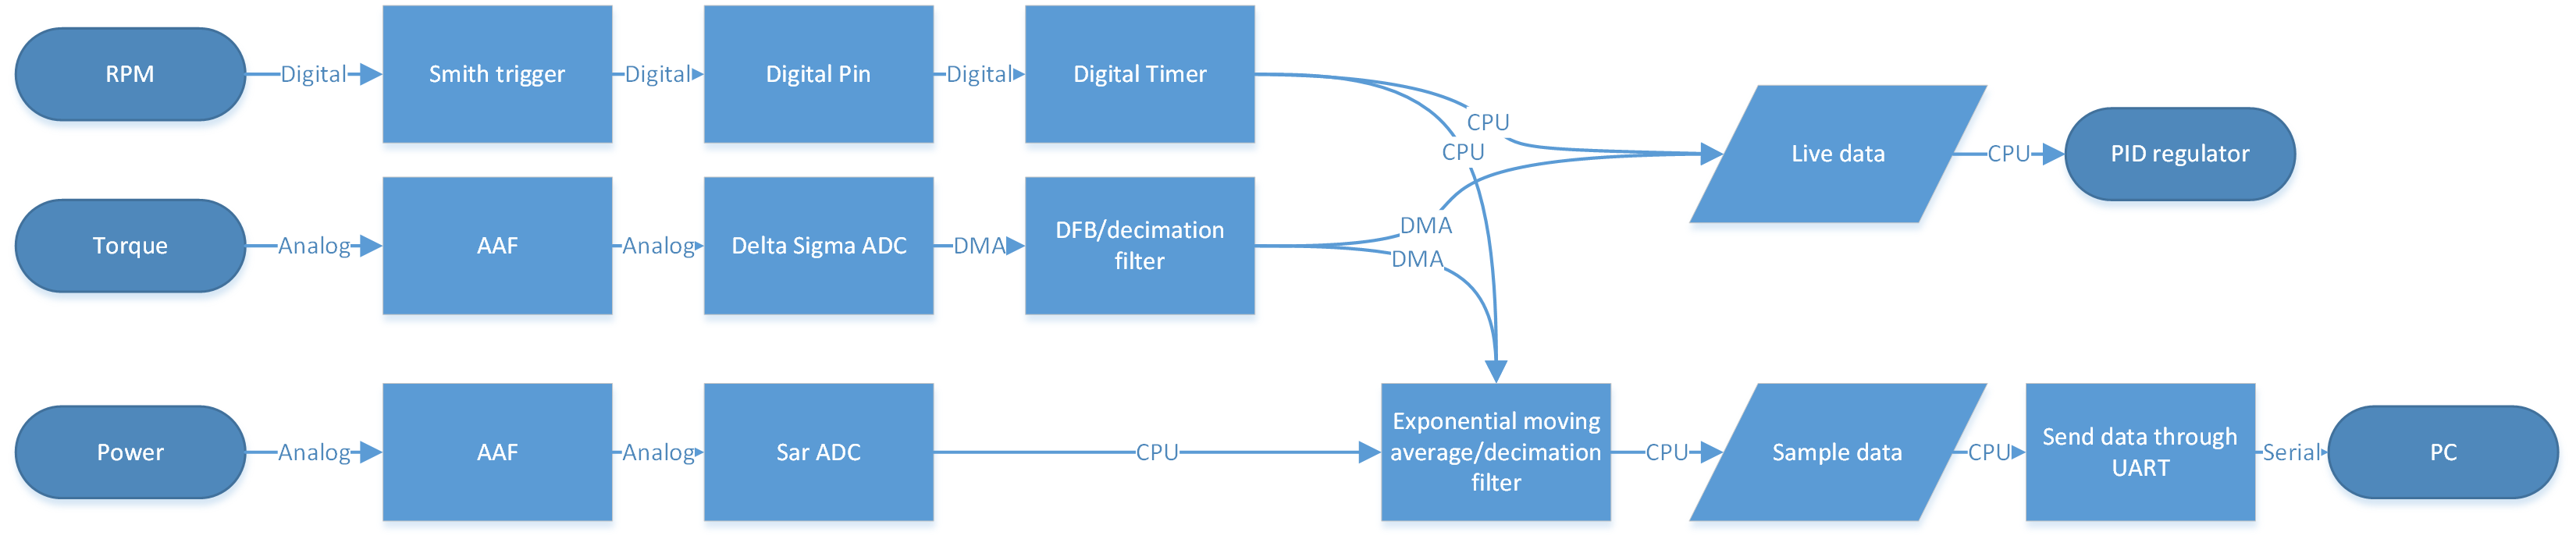
\includegraphics [width=6in]{../Documentation_RR/Software/Pictures/data-flow.png}
	\caption{Rolling Road data-flow diagram.}
	\label{fig:data_flow_diagram}
\end{figure}
\subsection{Test}
To test Rolling Road a test stand was setup with a test car figure \ref{fig:RR_first_test}. Where the measure of the car was made. 
\begin{figure}[H]
	\centering
	\includegraphics [width=3in]{SubPages/Images/jens_test.png}
	\caption{First test of the old AU car.}
	\label{fig:RR_first_test}
\end{figure}
After a half hour test a efficiency diagram could be made from the data \ref{fig:RR_first_test_result}.

\begin{figure}[H] 
	\centering
	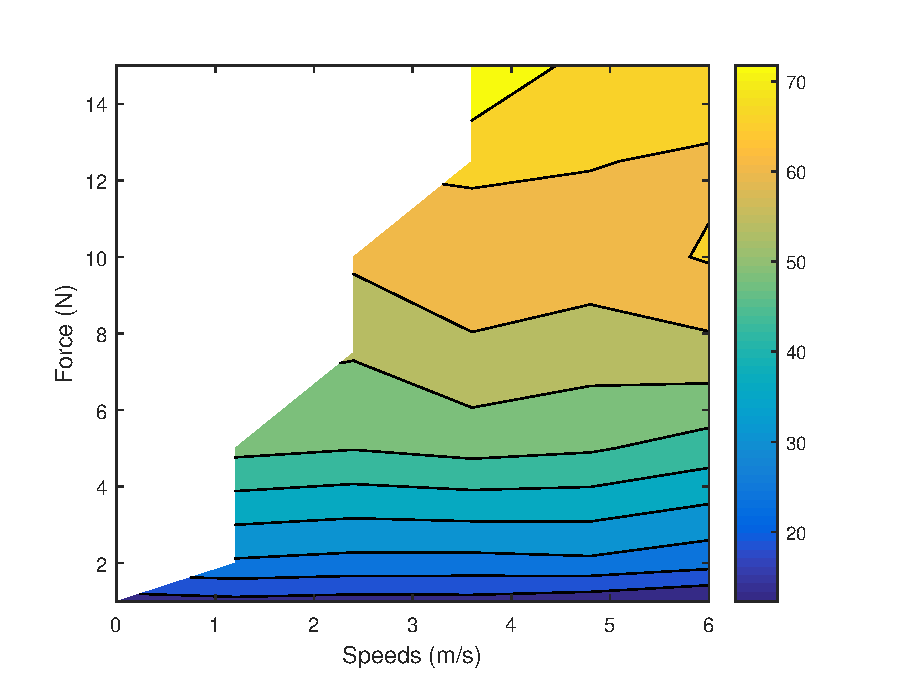
\includegraphics [width=3in]{SubPages/Images/RR_test_result.eps}
	\caption{efficiency diagram of the first test, the value is in \% efficiency.}
	\label{fig:RR_first_test_result}
\end{figure}
This result is not close enough to the efficiency what was calculated by a mechanical-engineer \cite{BAC_zenith33}. But the car is not in the best shape, and it was not fastened to the Rolling Road. So there is many places there is efficiency lost.


